%\NeedsTeXFormat{LaTeX2e} 
%%% check whether we are running pdflatex
% http://www.db.informatik.uni-bremen.de/~mr/pdflatex.html
%	\newif\ifpdf
%	\ifx\pdfoutput\undefined
%	  \pdffalse % we are not running pdflatex
%	\else
%	  \pdfoutput=1 % we are running pdflatex
%	  \pdfcompresslevel=9     % compression level for text and image;
%	  \pdftrue
%	\fi

%%% choose global options depending on whether
%%% we are running under pdflatex
	
%	\ifpdf
%\ifx\pdfoutput
%\documentclass[pdftex,a4paper,10pt,makeidx]{article}
%\documentclass[pdftex,a4paper,10pt,makeidx]{book}
%\documentclass[pdftex,a4paper,12pt]{book}
%\documentclass[pdftex,a4paper,12pt]{report}
%\documentclass[pdftex,a5paper,9pt]{book}
%\documentclass[pdftex,a4paper,11pt]{book}
\documentclass[pdftex,a4paper,12pt]{book}   % DISS
%\documentclass[pdftex,a4paper,12pt]{article} % List of publications
%	\else
%\fi
%\ifx\pdfoutput\undefined
%	  \documentclass[dvips,a4paper,10pt,makeidx]{article}
%\fi

% WINDOWS: use sumatra pdfviewer with TeXnicCenter to do inverse search
%http://www.wi.uni-muenster.de/qm/studieren/LaTeXVorlage.html
\usepackage{pdfsync}  % comment out for final document

\usepackage{ifpdf}  % uses oberdiek, cannot be used before documentclass
\usepackage{etex}  % Without there will be many "No room for a new \dimen" errors
\usepackage{a4}
\usepackage[T1]{fontenc}                      % EC-Schriften("richtige"Umlaute)
\usepackage[latin1]{inputenc}                 % Input coding
%\usepackage[utf8]{inputenc}                 % Input coding

%\renewcommand\appendixname{}%    "
\renewcommand\figurename{Fig.}
\renewcommand\tablename{Tab.}
%\usepackage{csquotes} % consistent quoting by \enquote{...}, without use \lq xyz\rq or \lqq xyz \rqq
% TABLES
%\usepackage{array,booktabs}
\usepackage{upgreek}
\usepackage{ulem} % provides \sout  strikeout
\normalem % restore italics for emph   
\usepackage{pifont}  % checkmark = \ding{52}
\usepackage{textcomp} % provides \textnumero
\usepackage{txfonts} % gammaup, upright greek characters
\usepackage{booktabs}       % Nicer Tables, provides \toprule, \midrule, \bottomrule
\usepackage{longtable}
\usepackage{multirow}% added090731, \multirow{3}{*}{content}, * for width
%\usepackage{ltablex}
%\usepackage{tabulary}% 
%\usepackage{ltxtable}% longable meet tabularx
%\usepackage{tools}

%\usepackage{sfheaders}              % SansSerif Font f�r �berschriften / for headings
\usepackage{pictex}                 % Plot-Paket
\usepackage{anysize}               % Uses full page, all of papersize, looks bad!
%\usepackage{fullpage}
\usepackage{xspace}                 % provides \xspace
%\usepackage[pdftex]{lscape}                 % Provides \begin{landscape} environment
\usepackage{pdflscape}                 % Provides \begin{landscape} environment
%%%%%%%%%%%%%%%%%%%%%
\usepackage{graphicx}               % PS-diagram package of pictures merge
%\usepackage[draft]{graphicx}        % PS-Grafikpaket nur Rahmen
%%%%%%%%%%%%%%%%%%%%%
\usepackage{psfrag}                 % PS-Text durch LaTeX-Code ersetzen
%\usepackage{draftstamp}    %%%%%%%%%% Entwurfstempel; draftstamp.sty %%%%%%%%%%%%%%%%%
\usepackage{placeins}        % definiert Floatsperre \FloatBarrier; placeins.sty
\usepackage[indent,bf]{caption}    % Einstellen des caption-Stils, war caption2
%\captionindent2em                   % Ma� f�r Einzug
% Workaround for backcite problem 
\usepackage{makerobust} 
\makeatletter 
\@ifundefined{caption@xref}{}{% 
  \MakeRobustCommand\caption@xref 
} 
\makeatother 
%I have notified the author of the caption package. 
%Yours sincerely 
%  Heiko <oberd...@uni-freiburg.de>

% Workaround against double definition error by using amssymb and txfonts:iint
\let\iint\dadada
\let\iiint\dadadaa
\let\iiiint\dadadab
\let\idotsint\dadadac

\usepackage{exscale}                % richtig skalierte Operatoren in Formeln
\usepackage{amsmath}                % Mathematik-Erweiterungen der AMS
\usepackage{amssymb}                % Mathematik-Erweiterungen der AMS
%\usepackage{onlyamsmath}
% ftp://tug.ctan.org/pub/tex-archive/info/Free_Math_Font_Survey/survey.html
%\usepackage{concmath}                %
%\usepackage{mathtime}
%\usepackage{mnsymbol}                 % incompatible with amssymb & amsfonts, pixelig, neswarrows
%\usepackage{cmbright}
%\usepackage{mathpazo}								% funktioniert
\usepackage{times}                  % von elsart abgeschaut
%\usepackage[math]{anttor}
%\usepackage{millennial}
%\usepackage{fouriernc}              % sch�neres gamma
%\usepackage{yhmath}								%
\usepackage{mathrsfs}               % for mathscr (Schreibschrift)
%\usepackage[math]{isomath}

%\ptexnoligatures%\textfont0 % bewirkt angebl. Unterdr�ckung von Ligaturen und kerning in pdftex

\usepackage{afterpage}              % Befehlsausf�hrung erst am Seitenende
\usepackage{natbib}                 % ein natbib-Stil, der auch bei author-year eine
% biblabel Marke im Literaturverzeichnis aufweist!
% natbib.sty ruft eine eigene Konfiguration natbib.cfg auf

\usepackage{xcolor}
\definecolor{lbcolor}{rgb}{0.9,0.9,0.9}
\definecolor{lightgrey}{rgb}{0.85,0.85,0.85} %
\definecolor{gray}{rgb}{0.5,0.5,0.5}% gray=AE, grey=BE
\definecolor{grey}{rgb}{0.5,0.5,0.5}% gray=AE, grey=BE

\usepackage{upgreek}

% KOPF- UND FUSSZEILEN
\usepackage{fancyhdr}        % Erwieterte Optionen f�r
\pagestyle{fancy}            % Kopf- und Fu�zeilen
\fancyhf{}                   % Alle Felder leeren
%\fancyfoot{}\fancyhead{}     %CZ clear all fields
%\fancyfoot[ro,le]{\footnotesize\thepage}  % Seitenzahl au�en
%\fancyfoot[l]{\footnotesize\today}
% NUR SEITENZAHL
\fancyfoot[ro,le]{\footnotesize\thepage}%\\\textcolor{gray}{C.\,Zambaldi, \today}}   % Seitenzahl
% SEITENZAHL UND VERSION INFO
%\fancyfoot[ro,le]{\footnotesize\thepage\\\textcolor{gray}{C.\,Zambaldi, \today}}   % Seitenzahl

\fancyhead[ro]{\footnotesize{\leftmark} }    % Kapitel rechts auf geraden Seiten
\fancyhead[le]{\footnotesize{\rightmark} }   % Abschnitt links auf ungeraden Seiten%
%\fancyhead[ro]{\textsc{\small{\leftmark}}}  %Zambaldi  % Kapitel rechts auf geraden Seiten
%\fancyhead[le]{\textsc{}} %2005  % Abschnitt links auf ungeraden Seiten%
\setlength{\headheight}{15pt}% H�he der Kopfzeile (def012pt) wg der Linie
\renewcommand{\headrulewidth}{0pt} %def0.4pt
\renewcommand{\footrulewidth}{0pt} %def0pt
\renewcommand\chaptername{}      %fancyhdr: Kapitel�berschrift ohne "Kapitel"
%\renewcommand{\chaptermark}[1]{\markboth{\textsc{\chaptername\ \thechapter\ \ #1}}{}}
%\renewcommand{\chaptermark}[1]{\markboth{{\thepart-\thechapter\ \ #1}}{}}
\renewcommand{\chaptermark}[1]{\markboth{{\thechapter\ \ #1}}{}}
%\renewcommand{\chaptermark}[1]{\markboth{{\thechapter\ }}{}}
%\renewcommand{\chaptermark}{\empty}
%\markboth{Zambaldi}
\renewcommand{\sectionmark}[1]{\markright{{\thesection\ #1}}}% Kein Punkt hinter Kapitelnummern in Kopfzeile
%\renewcommand{\sectionmark}{\empty}
%\renewcommand{\chaptermark}[1]{}
%\renewcommand{\sectionmark}[1]{}
\fancypagestyle{plain}{% Redefine "plain" style (e.g. for 1st side of chapters)
\fancyhf{} % clear all header and footer fields
%\fancyfoot[l]{{\tiny \today}}
%\fancyfoot[ro,le]{\footnotesize\thepage}
}
% http://www-h.eng.cam.ac.uk/help/tpl/textprocessing/squeeze.html
%\usepackage[medium,compact]{titlesec} % fontsize sections...
\usepackage[small,compact]{titlesec} % fontsize sections...
%\usepackage{sectsty} % An alternative to titlesec

%\titleformat{\subsection}{\normalfont\normalsize\bfseries}{\thesubsection}{1em}{} %bfseries to add bold style
%\titleformat{\subsubsection}%{\normalfont\normalsize\mdseries\itshape}{\thesubsubsection}{1em}{}
%\titleformat{\subsubsection}{\normalfont\normalsize\bfseries}{\thesubsubsection}{1em}{}


% TABELLENBESCHRIFTUNG
%\usepackage[tableposition=top]{caption}

% EINHEITEN
\usepackage{units}
% \unit[<wert>]{<einheit>}
% \unitfrac[<wert>]{<z�hler>}{<nenner>} 	
% \nicefrac[<schrift>]{<z�hler>}{<nenner>}

% MILLERSCHE INDICES
\usepackage{miller} % \hkl(123), \hkl<1 2 -3>, change spacing, with 
%\renewcommand{\millerskip}{\,\,\,}

% DOPPELTER ZEILENABSTAND mit \doublespace, weitere
\usepackage{setspace}
\singlespace % \singlespace, \onehalfspace, \doublespace

% LISTINGS; Quellcode einbinden und formatieren.
\usepackage{listings}       %[savemem]{listings}
\lstloadlanguages{fortran} %TeX %[LaTeX]TeX
\lstset{language={},
  frame=none,
  xleftmargin=10mm,
  xrightmargin=10mm,
	numbers=left,
	stepnumber=1,
	numbersep=5pt,
	numberstyle=\tiny,
	breaklines=true,
	breakautoindent=true,
	postbreak=...,%\space,
	tabsize=2,
	basicstyle=\ttfamily\footnotesize,
	showspaces=false,
	showstringspaces=false,
	extendedchars=true,
	backgroundcolor=\color{white}
}

% ---------------------------------------------------------------------------

% BILD�BERLAGERUNG
%\usepackage[abs]{overpic} % [percent]

%\usepackage{calc}

% PARAGRAPH INDENTATION AND VERTICAL SPACE
\setlength{\parindent}{0pt}                              % kein Einzug am Absatz
%\parskip 1.0ex plus 0.2ex minus 0.2ex                    % Abstand Absatz FR:1.5ex plus 0.5ex minus 0.5ex
\setlength\parskip{.5\baselineskip
	plus .1\baselineskip
	minus .4\baselineskip
}

\sloppy                                                  % Seitenende "schlampig"
\setcounter{secnumdepth}{3}                              % Abschnitts-Num.tiefe(def=2)
\setcounter{tocdepth}{3}                       % Inhaltsverzeichnistiefe (def=2)
\setcounter{bottomnumber}{2}                   % Max. Gleitobjekte unten (def=1)
\setcounter{totalnumber}{4}                    % Max. Gleitobjekte insg.  (def=3)
\renewcommand{\topfraction}{0.75}              % Max. rel. Platz f�r Gleitobjekte
\renewcommand{\bottomfraction}{0.65}           % oben bzw. unten (def=0.7 bzw. 0.3)
\newcommand{\versetzung}[1]{\rotatebox{#1}{\rule[-2mm]{0cm}{4mm}\tiny $\bot$}}    % Versetzungssymbol{Winkel}
\newcommand{\vernull}{\tiny $\bot$}            % Versetzungssymbol 0 Grad
\newcommand{\vereinsachtnull}{\tiny $\top$}    % Versetzungssymbol 180 Grad
\newcommand{\verneunnullp}{\tiny $\dashv$}     % Versetzungssymbol 90 Grad
\newcommand{\verneunnullm}{\tiny $\vdash$}     % Versetzungssymbol -90 Grad
%\newcommand{\RX}{Rekristallisation}
%, als Dezimaltrennzeichen in Kommazahlen im Mathemodus
\mathchardef\CommaOrdinary="013B
\mathchardef\CommaPunct="613B
\mathcode`,="8000 %, im Math-Mode aktiv machen
{\catcode`\,=\active
 \gdef,{\obeyspaces\futurelet\next\CommaCheck}}
\def\CommaCheck{\if\space\next\CommaPunct\else\CommaOrdinary\fi}

%\def\figurename{} % Fig. oder Abb.								
\makeatletter                                                   % @ define as normal letters
\def\cleardoublepage{\clearpage \if@twoside \ifodd\c@page       % with CLEAR double PAGE second side empty
                     \else \hbox{} \thispagestyle{empty} \newpage
                     \if@twocolumn \hbox{} \newpage \fi \fi \fi}
%\renewcommand\part{%               % with part first side empty
%  \if@openright
%    \cleardoublepage
%  \else
%    \clearpage
%  \fi
%  \thispagestyle{empty}%
%  \if@twocolumn
%    \onecolumn
%    \@tempswatrue
%  \else
%    \@tempswafalse
%  \fi
%  \null\vfil
 % \secdef\@part\@spart}
%\makeatother         % @ again as other indication define

% Upright greek characters: http://www.superstrate.net/useful/useful.html
\DeclareFontFamily{U}{euc}{}% I chose euc because the chart is called Euler cursive 
\DeclareFontShape{U}{euc}{m}{n}{<-6>eurm5<6-8>eurm7<8->eurm10}{}% 
\DeclareSymbolFont{AMSc}{U}{euc}{m}{n} % I chose AMSc because AMSa and AMSb are defined in the amsfonts-package 
\DeclareMathSymbol{\umu}{\mathord}{AMSc}{"16}


% HYPERREF   package definition
\usepackage{color}
\definecolor{lnkcol}{rgb}{0, .1, .5}
\definecolor{lnkcol}{rgb}{0, .1, .5}


%\ifpdf

%\usepackage{pstricks, pst-plot}

\ifpdf   % IFPDF
  %\usepackage[pdftex]{thumbpdf}      %%% thumbnails for ps2pdf
%\usepackage[ps2pdf]{hyperref}
  \usepackage[pdftex,                %%% hyper-references for ps2pdf
%backref=section,											 %%% bibliographical backlinks
pagebackref=true,	                 %%% links in bibliography to pages
bookmarks=true,%                   %%% generate bookmarks
bookmarksnumbered=false,           %%% numbered bookmarks on/off
bookmarksopen=true,                %%% bookmarkstree open/closed
hypertexnames=false,%              %%% needed for correct links to figures!
breaklinks=true,%                  %%% break lines on/off, on => links can become very small
pdfborder=false,                   %%% Links mit Rahmen on/off
pdfpagelabels=true,								 %%% logische/physikalische Seitenzahlen true/false*
pdftoolbar=true,									 %%% Men�leisten true*/false	
linkbordercolor={1 1 1},%    %%% color of frames around links
citebordercolor={1 1 1},
urlbordercolor={0.8 0.8 .8},
colorlinks=true,
linkcolor=lnkcol, % black, blue, red, green, cyan, ...
urlcolor=lnkcol,%{.2 .2 1},
citecolor=black,
]{hyperref} %HYPERREF

% PDF METAINFORMATION
  \hypersetup{
pdfauthor   = {},
pdftitle    = {},
pdfsubject  = {},
pdfkeywords = {},
pdfcreator  = {},
pdfproducer = {pdftex}%,
%pdfpagemode={FullScreen}
}

% ATTACH ARBITRAY FILES TO THE RESULTING PDF. FILES ARE STORED INSIDE OF THE PDF-FILE.
%\usepackage{attachfile}  % Only with pdftex. Makes use of "oberdiek" package
%\attachfilesetup{color=0 .1 .5}


  \usepackage{pst-pdf} % pstricks for pdflatex

\else
  \usepackage{pstricks, pst-plot}
  \usepackage[hypertex]{hyperref}
\fi

\usepackage{textcomp} %Dieses Paket enthaelt die Befehle %\textdegree%\textcentigrade%und eine Menge anderer nuetzlicher Symbole.


% MULTIPLE BIBLIOGRAPHIES
%\usepackage{bibunits}

%\usepackage{makeidx}
%\makeindex

%%%%%%%%%%%%%%%%%%%%%%%%%%%%%%%%%%%%%%%%%%%%%%%%%%%%%%%%%
%%%%%%%%%%% END OF HEADERFILE %%%%%%%%%%%%%%%%%%%%%%%%%%%
%%%%%%%%%%%%%%%%%%%%%%%%%%%%%%%%%%%%%%%%%%%%%%%%%%%%%%%%% 
%\listfiles% outputs info about packages
\bibpunct{(}{)}{,}{}{,}{,} % Zitierstil: {start}{ende}{multi-sep}{}{}...

\newcommand{\marcinput}{<model>\_<job>.dat\xspace}

\begin{document}
% BLANK SPACES BEFORE AND AFTER SECTIONS ...
% \@startsection {NAME}{LEVEL}{INDENT}{BEFORESKIP}{AFTERSKIP}{STYLE}
%            optional * [ALTHEADING]{HEADING}
%    Generic command to start a section.
%    NAME       : e.g., 'subsection'
%    LEVEL      : a number, denoting depth of section -- e.g., chapter=1,
%                 section = 2, etc.  A section number will be printed if
%                 and only if LEVEL < or = the value of the secnumdepth
%                 counter.
%    INDENT     : Indentation of heading from left margin
%    BEFORESKIP : Absolute value = skip to leave above the heading.
%                 If negative, then paragraph indent of text following
%                 heading is suppressed.
%    AFTERSKIP  : if positive, then skip to leave below heading,
%                       else - skip to leave to right of run-in heading.
%    STYLE      : commands to set style
%  If '*' missing, then increments the counter.  If it is present, then
%  there should be no [ALTHEADING] argument.  A sectioning command
%  is normally defined to \@startsection + its first six arguments.

%\renewcommand\section{\@startsection {section}{1}{\z@}{-3.5ex plus -1ex minus
%    -.2ex}{2.3ex plus .2ex}{\Large\bf}}
\renewcommand\subsection{\@startsection{subsection}{2}{\z@}{-.5ex plus -.2ex minus
   -.2ex}{.3ex plus .2ex}{\large\bf}} %\large\bf
\renewcommand\subsubsection{\@startsection{subsubsection}{3}{\z@}{-.5ex plus
-1ex minus -.2ex}{.2ex plus .5ex}{\normalsize\bf}}%\bf}}
%\renewcommand\paragraph{\@startsection
%     {paragraph}{4}{\z@}{3.25ex plus 1ex minus .2ex}{-1em}{\normalsize\bf}}
%\renewcommand\subparagraph{\@startsection
%     {subparagraph}{4}{\parindent}{3.25ex plus 1ex minus
%     .2ex}{-1em}{\normalsize\bf}}
%\renewcommand{\subsection}{\newpage \subsection}

% LaTeX spezigfisch
\def\ctr{\centering }

%Textmakros (Deutsch)
\def\bzw{bzw\. }

%Textmakros (Englisch)
\def\eg{e.\,g.\@\xspace}
\def\ie{i.\,e.\@\xspace}
\def\cf{c.\,f.\@\xspace}

%\renewcommand\lq{\lq\xspace}
%\renwecommand\rq{\rq\xspace}

% TABELLEN
\def\midruleI{\midrule[\heavyrulewidth]}

% Allgemein
\def\etal{et.~al.\xspace}
\newcommand{\superscript}[1]{\ensuremath{^\textrm{#1}}}
\newcommand{\subscript}[1]{\ensuremath{_\textrm{#1}}}
\def\verweis{$\uparrow$}

% Track changes in a document
\definecolor{addColor}{rgb}{0, .5, .0}
\definecolor{delColor}{rgb}{.6, .0, .0}
\newcommand{\add}[1]{\cbstart{}\textcolor{addColor}{\uline{#1}}\cbend{}\xspace}  
\newcommand{\del}[1]{\cbdelete{}\textcolor{delColor}{\sout{#1}}\xspace}  
% Cannot be used in captions so far /!\
%\newcommand{\add}[1]{#1\xspace}  \newcommand{\del}[1]{#1\xspace}  
\newcommand{\rep}[2]{\del{#1}\add{#2}}  
\newcommand{\done}{\ding{52}\xspace}


% INDENTATION
\def\max{\subscript{max}}
\def\Pmax{$P$\hspace{-.3em}\subscript{max}}
\def\hmax{$h$\subscript{max}}
\def\projA{\ensuremath{A\hspace{-0.2em}_{\perp}}\xspace}

% Figure and Table references
% see also the autoref command from hyperref package
\def\Chapref#1{Chapter~\ref{ch:#1}}
\def\chapref#1{chapter~\ref{ch:#1}}
\def\figref#1{figure~\ref{fig:#1}}
\def\tabref#1{table~\ref{tab:#1}}
\def\Figref#1{Figure~\ref{fig:#1}}
\def\Tabref#1{Table~\ref{tab:#1}}

%\newcommand{\deg}{\ensuremath{^{\circ}}}

% Mathe                  
% \upright 
\newcommand{\bsym}[1]{\ensuremath{\boldsymbol{#1}}} % \boldsymbol,\mathbb (blackbord bold), mathsf
%\def\tens{\boldsymbol}
\newcommand{\bsymIV}[1]{\ensuremath{\boldsymbol{\mathbb{#1}}}}
%\newcommand{\bsymIV}[1]{\boldsymbol{\mathcal{#1}}}
%\newcommand{\bsymIV}[1]{\boldsymbol{\mathscr{#1}}}
\newcommand{\tensII}[1]{\bsym{#1}}   % tensor of rank 2
\newcommand{\tensIV}[1]{\bsymIV{#1}} % tensor of rank 4
\def\kron{\delta}
\def\grad{\text{grad\,}} %gradient
 
% Symbole
\def\paralleldir{\ensuremath{\nearrow\hspace{-.4em}\nearrow}\xspace}
\def\antiparalleldir{\ensuremath{\nearrow\hspace{-.4em}\swarrow}\xspace}

% MECHANIK
\def\sig{\ensuremath{\sigmaup}}
\def\eps{\ensuremath{\varepsilonup}}
\def\strain{\ensuremath{\tensII{\varepsilonup}}}
\def\stress{\ensuremath{\tensII{\sigmaup}}}
\def\hpu{MPa\hspace{-.1em}\ensuremath{\sqrt{\text{m}}}\xspace}%$^{-0.5}$} % Hall-Petch unit for k (slope)


\def\PK2{\ensuremath{\bsym{T}}}

%KRISTALLPLASTIZITAET
\def\burgers{\ensuremath{\bsym{b}}\xspace}
\def\bOD{\ensuremath{\burgers^{\text{O}}}\xspace}
\def\bSU{\ensuremath{\burgers^{\text{S}}}\xspace}
\def\bTW{\ensuremath{\burgers^{\text{T}}}\xspace}

% MaWi
\def\atpct{at.\%\xspace}
\def\gmat{\ensuremath{\tensII{g}}\xspace} % orientation matrix

% Kristallo
\newcommand{\angaxis}[2]{#1-around-#2\xspace}

% Bunge Euler Angles
\def\beaphiI{\ensuremath{\varphi_1}}
\def\beaPhi{\ensuremath{\it{\Phi}}}
\def\beaphiII{\ensuremath{\varphi_2}}
\def\BEAs{\ensuremath{(\beaphiI, \beaPhi, \beaphiII)}\xspace}
% Euler winkel
\def\pI{\ensuremath{\beaphiI}}
\def\pII{\ensuremath{\beaphiII}}

%\def\fcc{f.c.c.\xspace}
%\def\bcc{b.c.c.\xspace}
%\def\hcp{h.c.p.\xspace}
\def\fcc{fcc\xspace}
\def\bcc{bcc\xspace}
\def\hcp{hcp\xspace}
%\def\fcc{FCC\xspace}
%\def\bcc{BCC\xspace}
%\def\hcp{HCP\xspace}

% Mikrometer, microns
\def\mum{\ensuremath{\muup}m\xspace}


% TiAl 
%\def\gam{\ensuremath{\upgamma}}
\def\gam{\texorpdfstring{\ensuremath{\gammaup}}{gamma}\xspace} % requires txfonts package
\def\cgamma{\ensuremath{c_{\gam}}}
\def\agamma{\ensuremath{a_{\gam}}}

\def\gTiAl{\texorpdfstring{\mbox{\gam-TiAl}}{gamma-TiAl}\xspace}
\def\gammaTiAl{\gTiAl}
\def\caratio{$c\hspace{-1.pt}/\hspace{-1.5pt}a$\;ratio\xspace}
%alpha_2-Ti_3Al
\def\alptwo{\texorpdfstring{\ensuremath{\upalpha_2}}{alpha2}\xspace}
%\def\tiala2{$\alpha_2$-Ti$_3$Al}
%\def\tiala2{$\alpha_2$-Ti$_3$Al}

%\def\a2ti3al{$\alpha_2$-Ti$_3$Al}
%\def\a2Ti3Al{$\alpha_2$-Ti$_3$Al}
%\def\aIIti3al{$\alpha_2$-Ti$_3$Al}
%\providecommand{\aTi3Al}{\mbox{$\alpha$-Ti$_3$Al}}
\def\a2Ti3Al{\alptwo-Ti\texorpdfstring{$_3$}{3}Al\xspace}
%\providecommand{\a2ti3al}{{$\alpha_2$-Ti$_3$Al}}
%Ti_3Al
\def\Ti3Al{\a2Ti3Al}
\def\ti3al{\a2Ti3Al}
%\def\a2{$\alpha_2$}
%\def\taucO{\ensuremath{\tau_{c,O}}\xspace}
%\def\taucS{\ensuremath{\tau_{c,S}}\xspace}
%\def\taucT{\ensuremath{\tau_{c,T}}\xspace}
\def\taucO{\ensuremath{\tau_{c}^{O}}\xspace}
\def\taucS{\ensuremath{\tau_{c}^{S}}\xspace}
\def\taucT{\ensuremath{\tau_{c}^{T}}\xspace}

\def\LamAng{\ensuremath{\varPhi_{\text{L}}}\xspace}
\def\MatrixI{M1\xspace}
\def\MatrixII{M2\xspace}
\def\MatrixIII{M3\xspace}
\def\TwinI{T1\xspace}
\def\TwinII{T2\xspace}
\def\TwinIII{T3\xspace}


%% Strukturbericht % http://cst-www.nrl.navy.mil/lattice/
\def\L10{L1$_0$\xspace}
\def\D019{D0$_{19}$\xspace} % 0 (zero) not O

\newcommand\half{\ensuremath{\nicefrac{1}{2}}}
\newcommand\sixth{\ensuremath{\nicefrac{1}{6}}}
\newcommand\nr{no.\,}



\newpage
\thispagestyle{empty}
%\headrule
\begin{center} 
\vspace*{.1\textwidth}
%{\bf 
{\huge
Manual to the\\ Crystal Plasticity Finite Element Subroutine\\ developed at the\\ Max-Planck-Institut f�r Eisenforschung\\}

\vfill
\today
%\\[0.4ex] 
%\gTiAl based alloys}
%-TiAl based alloys}
%\vspace{10ex}

%%%%Von der Fakult�t f�r Bergbau, H�ttenwesen und Geowissenschaften\\ % bewilligt
%%%%Der Fakult�t f�r Bergbau, H�ttenwesen und Geowissenschaften\\ % einreichung
%Von der Fakult�t f�r Georessourcen und Materialtechnik\\ % bewilligt
%Der Fakult�t f�r Georessourcen und Materialtechnik\\ % einreichung
%[2ex]
%der Rheinisch-Westf�lischen Technischen Hochschule Aachen\\[6ex]
%zur Erlangung des akademischen Grades eines\\[2ex]
%Doktors der Ingenieurwissenschaften genehmigte\\ % bewilligt
%Doktors der Ingenieurwissenschaften vorgelegte\\ % einrichung
%[5ex]
%{\large Dissertation}\\
%[5ex]
%vorgelegt %bewilligt
%von Diplom-Ingenieur\\
%[5ex]
%{\large Claudio Zambaldi}\\
%[5ex]
%aus M�nchen
\end{center}
% REST: Pflichtexemplar
%\vfill
%\begin{tabbing}
%Berichter:\hspace{1cm}\=Professor Dr.-Ing. D. Raabe\\
%\>Universit�tsprofessor Dr. rer. nat. G. Gottstein
%\end{tabbing}
%
%Tag der m�ndlichen Pr�fung: %?.?.2010
%
%Diese Dissertation ist auf den Internetseiten der Hochschulbibliothek online verf�gbar.
\newpage
%\thispagestyle{empty}
%\headrule
\begin{center} 
\vspace*{.1\textwidth}
%{\bf 
{\huge
Manual to the\\ Crystal Plasticity Finite Element Subroutine\\ developed at the\\ Max-Planck-Institut f�r Eisenforschung\\}

\vfill
\today
%\\[0.4ex] 
%\gTiAl based alloys}
%-TiAl based alloys}
%\vspace{10ex}

%%%%Von der Fakult�t f�r Bergbau, H�ttenwesen und Geowissenschaften\\ % bewilligt
%%%%Der Fakult�t f�r Bergbau, H�ttenwesen und Geowissenschaften\\ % einreichung
%Von der Fakult�t f�r Georessourcen und Materialtechnik\\ % bewilligt
%Der Fakult�t f�r Georessourcen und Materialtechnik\\ % einreichung
%[2ex]
%der Rheinisch-Westf�lischen Technischen Hochschule Aachen\\[6ex]
%zur Erlangung des akademischen Grades eines\\[2ex]
%Doktors der Ingenieurwissenschaften genehmigte\\ % bewilligt
%Doktors der Ingenieurwissenschaften vorgelegte\\ % einrichung
%[5ex]
%{\large Dissertation}\\
%[5ex]
%vorgelegt %bewilligt
%von Diplom-Ingenieur\\
%[5ex]
%{\large Claudio Zambaldi}\\
%[5ex]
%aus M�nchen
\end{center}
% REST: Pflichtexemplar
%\vfill
%\begin{tabbing}
%Berichter:\hspace{1cm}\=Professor Dr.-Ing. D. Raabe\\
%\>Universit�tsprofessor Dr. rer. nat. G. Gottstein
%\end{tabbing}
%
%Tag der m�ndlichen Pr�fung: %?.?.2010
%
%Diese Dissertation ist auf den Internetseiten der Hochschulbibliothek online verf�gbar.
\cleardoublepage \phantomsection % set the hyperref anchor at the right position
\addcontentsline{toc}{section}{Table of contents} %
\tableofcontents
%\listoftables \addcontentsline{toc}{section}{Tables} %
%\listoffigures \addcontentsline{toc}{section}{Figures} %\newpage
\renewcommand{\chaptermark}[1]{\markboth{{\thechapter\ \ #1}}{}}

\chapter{Preliminaries}
\section{Introduction}
For the theory and some application examples, see \citet{Roters2010}.

\section{History of the code}
?, spaghetti version, 

\section{Accessing the version controlled subroutine}
% This section is copied from the msuwiki: http://msusrv4/msuwiki/Theory%20and%20Simulation/SVN
Before you start: Before you are able to access the version-controlled software, you need to get a valid login to the msuhp9 server. Please ask either Berthold Becksch\"afer (-922) or Achim Kuhl (-923) to set up your permissions accordingly. 

\subsection{Windows}
\subsubsection{Putty}
Get yourself PuTTY and PuTTYgen from http://www.chiark.greenend.org.uk/~sgtatham/putty/download.html 
Generate a RSA (SSH2) 2048 bit strong key pair with PuTTYgen. Save the private part of the key to a secure location (My Documents or such). Copy the public part from the PuTTYgen window, paste it into a text-editor and save. Append the contents of that file to \verb|~/.ssh/authorized_keys| on any workstation you can log on to. 
Create a profile in PuTTY called "msuhp9" with host: msuhp9.mpie.de, your standard "MPIE\\myName" username and specify the above location of your private key file as means of authentication. 
You should then be able to connect with this profile to msuhp9 WITHOUT password authentication! 

\subsubsection{Tortoise}
Install the subversion-client Tortoise at http://tortoisesvn.net/downloads 
Create a directory to hold the CPFEM subroutine on your PC. 

Right-Click in this folder and select "SVN checkout" from the context menu. Specify 
svn+ssh://msuhp9/home/svn/repos/cpfem

as the URL of the desired repository. This will use the profile named "msuhp9" from PuTTY and should hence not ask for any authentication from your end.

\subsection{Linux workstations}

\subsubsection{Key authentication}
if not already done, generate a 2048 bit RSA key pair using 
ssh-keygen -t rsa -b 2048 
and go for the standard options offered. This will create "id\_rsa" (private key) and "id\_rsa.pub" (public key) within your \verb|~/.ssh| folder.

Append \verb|id_rsa.pub| to \verb|~/.ssh/authorized_keys| and try logging into another workstation with 
ssh MPIE\\\\myName@msuwsX
(exchange X with 2...11). It should NOT require password authentication.

\subsubsection{Checkout}
create a directory to hold the subversion-controlled CPFEM routine and change into this. 
svn checkout svn+ssh://MPIE\\\\myName@msuhp9.mpie.de/home/svn/repos/cpfem
to copy the repository content to the current working directory -- done.

familiarize yourself with svn: svn help


\section{Style guide for programming the CPFEM subroutine}
Some hints
\begin{itemize}
\item This manual cannot substitute proper commenting in the Fortran code. Try to include as much comments as possible directly in the code. 
\item When commenting, do not use cryptic comments such as \emph{Random is random!} -- an actual
example from the code. 
\end{itemize}


\chapter{Organization of the code}


\begin{figure}
	\centering
		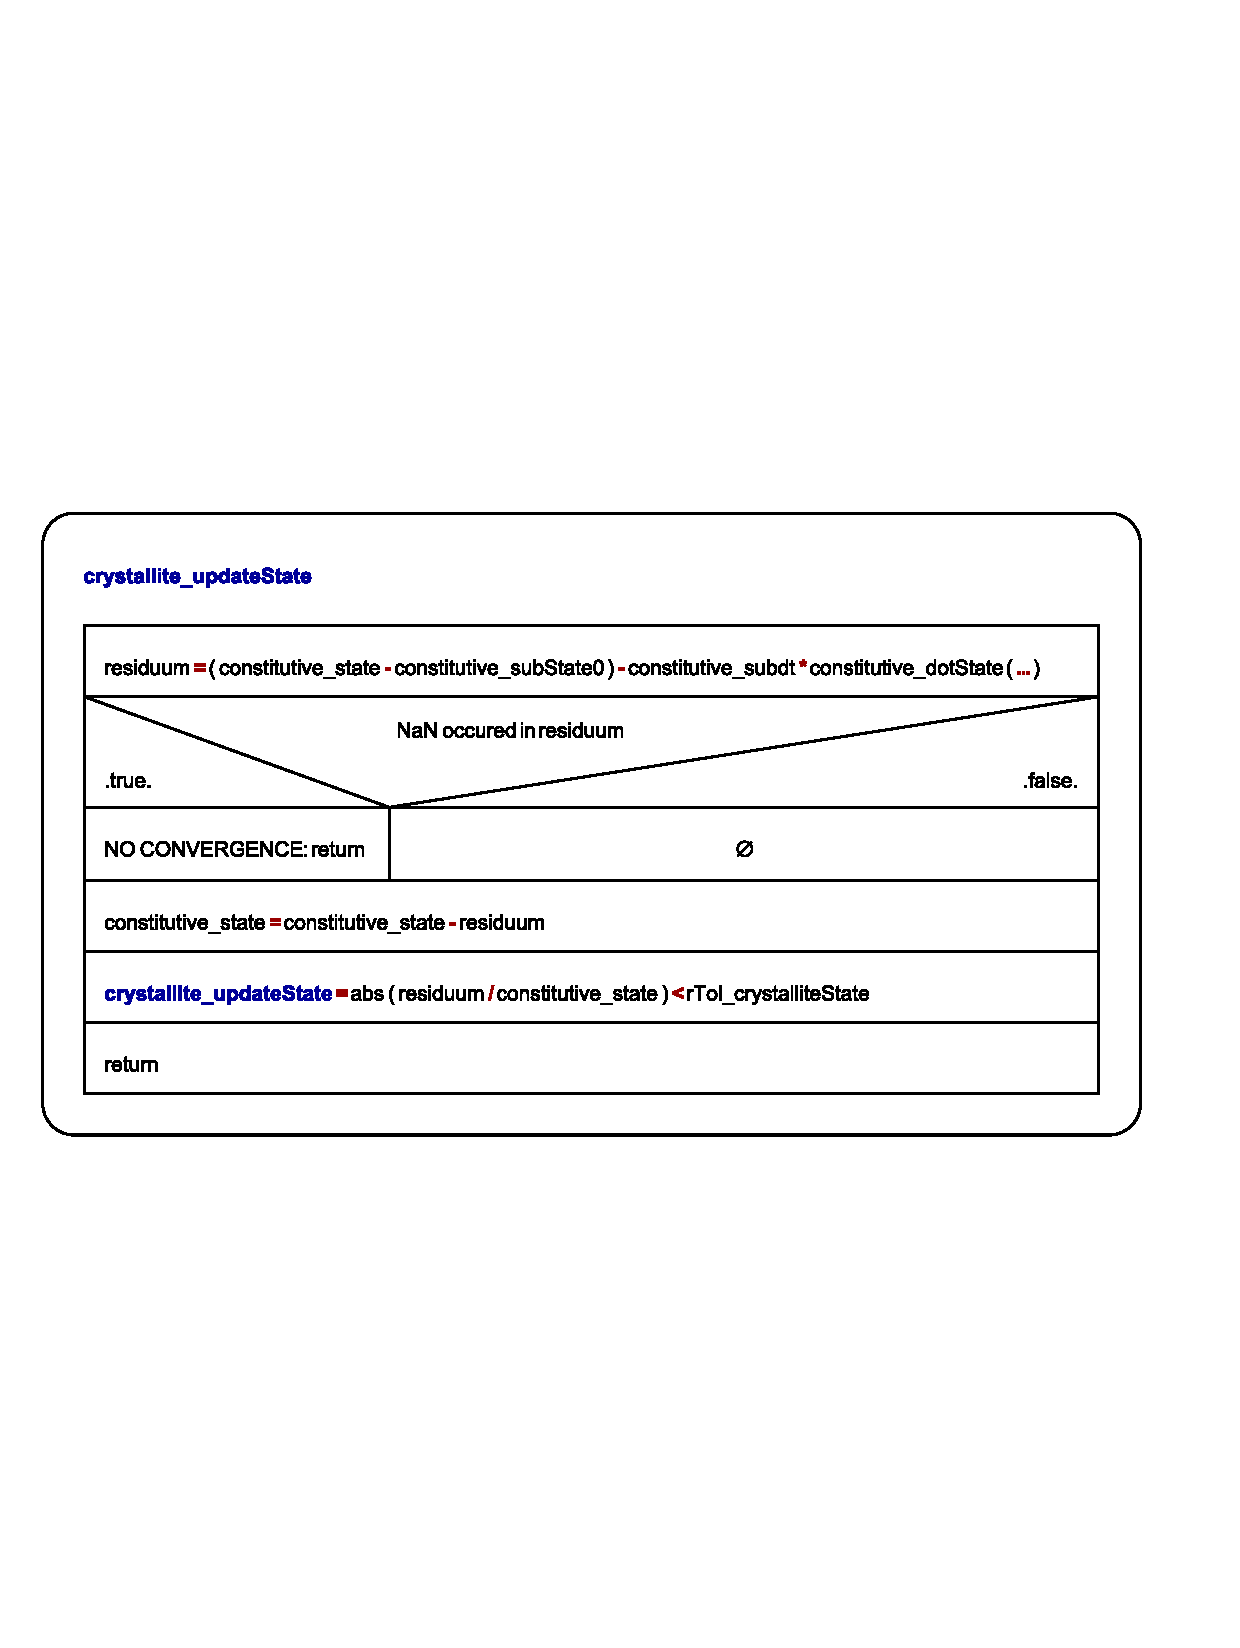
\includegraphics[width=0.80\textwidth]{../../cpfem/documentation/NSD/crystallite_updateState.pdf}
	\caption{updateState}
	\label{fig:crystallite_updateState}
\end{figure}


\chapter{Homogenization schemes}
%\section{Introduction}
If more than one grain is simulated per integration point, a homogenization scheme is required to distribute the deformation gradient of the IP to the respective grains. The simplest choice is the \emph{isostrain approach} which simply consists in assuming the IP deformation gradient to be applicable directly to each grain. 
%\section{Isostrain homogenization -- Taylor's assumption}
%\section{RGC}

cite RGC papers...

\chapter{Constitutive Laws}
\section{phenoPowerlaw}
\subsection{The material file for phenoPowerlaw}
\section{dislotwin}
\section{The non-local model}

\section{The material file: material.config}

\chapter{Application notes for different finite elements systems}
\section{MSC.MARC/Mentat}
In MARC the CPFEM routine is interfaced through the {\ttfamily hypela2} subroutine. The routine {\ttfamily makeMe.py} produces the interface files such as {\ttfamily mpie\_cpfem\_marc2008r1.f90} that will can be called by the different MARC releases. 

Necessary changes in the submit scripts

Model definition for using the subroutine: In MARC, state variable 1 defines the temperature in Kelvin. State variables 2 and 3 define the homogenization and microstructure, respectively.

Analysis options to invoke: Large Strain, Updated Lagrange. For most problems, using a constant dilatation formulation is important for robustness of the simulations. 
%The analysis options are most conveniently defined through a procedure file.

\subsection{Utility scripts}
\begin{itemize}
\item marcAddUserOutput.py [<No. of UserVars>] \marcinput --- adds UserVariables to the \marcinput file under the "post" section
\end{itemize}

\subsection{Practical hints}
A copy of the subroutine on the home directory on the SAN makes the routine accessible from all workstations under /san/arbitraryfoldername/code/*.f90 .
Under windows it is beneficial to keep an additional local copy of the routine to work with TortoiseSVN, since the change of folder icons seems to not work on the SAN. 


\section{Troubleshooting}
\subsection{Inside out element error}
An inside out element error can occur if the number of increment is chosen too small. This was observed for revision 539 using the pheno-powerlaw constitutive formulation on a particle in mesh problem. 

\section{Abaqus}
Differences to Marc.

\chapter{Postprocessing of the results}
mentat, py\_post, gri, ParaView, TSL-OIM

\chapter{Worked examples}
Refer to the corresponding publications ...



\appendix \addcontentsline{toc}{chapter}{Appendix}
\cleardoublepage \phantomsection % set the hyperref anchor at the right position

\fancypagestyle{plain}
{% Redefine "plain" style (e.g. for 1st side of chapters)
\fancyhf{} % clear all header and footer fields
\fancyfoot[ro,le]{\footnotesize\thepage}
}

\chapter{Crystallographic orientations}
\section{Bunge Euler angles}
\label{bunges}
Euler angles (\beaphiI, \beaPhi , \beaphiII) -- in Bunge convention -- rotate the sample coordinate system ($X$,~$Y$,~$Z$  or RD,~TD,~ND) into the crystal coordinate system ($x_c$, $y_c$, $z_c$). 
Three successive rotations are carried out in the following way \citep[pg.\,4]{Bunge1982}:
\begin{enumerate}
	\item Rotate by angle $\pI$ around Z, to bring X into the $x_c$--$y_c$-plane. The new intermediate axes are X', Y' and Z (Z is unchanged).
	\item Now rotate $\beaPhi$ degrees around X', to make Z parallel with $z_c$. The intermediate axes are X', Y'', Z'.
	\item A rotation by angle $\pII$ around Z' makes the rotated axes then identical to the crystal axes.
\end{enumerate}

The rotation matrix can be calculated as
\[% Gottstein pg 55
\bsym{g}=\left(\begin{array}{ccc}
\cos{\pI}\cos{\pII}-\sin{\pI}\sin{\pII}\cos{\beaPhi} & \sin{\pI}\cos{\pII}+\cos{\pI}\sin{\pII}\cos{\beaPhi}& \sin{\pII}\sin{\beaPhi}\\
-\cos{\pI}\sin{\pII}-\sin{\pI}\cos{\pII}\cos{\beaPhi} & -\sin{\pI}\cos{\pII}+\cos{\pI}\cos{\pII}\cos{\beaPhi}& \cos{\pII}\sin{\beaPhi}\\
\sin{\pI}\sin{\beaPhi} & -\cos{\pI}\sin{\beaPhi}& \cos{\beaPhi}
\end{array}\right)
\]

\newpage

\chapter{Related works}
\section{Publications}

\section{PhD thesises}
KuoDiss MaDiss ZaafaraniDiss
%
% Quellenverzeichnis
% http://www.cs.stir.ac.uk/~kjt/software/latex/showbst.html
%\bibliographystyle{} %
%\bibliographystyle{authordate3} %  EX: DEY, S.R., HAZOTTE, A., & BOUZY, E. 2006. Multiscale gamma variant selection in a quarternary near-gamma Ti-Al alloy. Philosophical Magazine, 86(20), 3089�3112.
%
%\bibliographystyle{chicago} %  EX: Appel and Christoph (1999) || Appel, F. and U. Christoph (1999). Coherency stresses and interface-related deformation phenomena in two-phase titanium aluminides. Intermetallics 7, 1173�1182.
%\bibliographystyle{elsarticle-num-names}
%
%\bibliographystyle{test} %see zambaldi/makebstTest/latex makebst
\bibliographystyle{diss_doi} %small manual changes from test.bst:
% doi linking, no ISSN for articles
%
%\bibliographystyle{spmpsci} % Springer
%\bibliographystyle{FRADINAT} %
%\bibliographystyle{abbrv} % [1], numbered
%\bibliographystyle{./bst/plainnat} % makes *everything* lower-case; plainnatm,abbrvnat,unsrtnat
%\bibliographystyle{./plainnat} % makes *everything* lower-case; plainnatm,abbrvnat,unsrtnat
% http://www.elisanet.fi/ptvirtan/misc/google-bibtex.html for doi linking
% Literaturverzeichnis
%\renewcommand{\bibname}{References} % default: Bibliography
\cleardoublepage \phantomsection % set the hyperref anchor
\addcontentsline{toc}{chapter}{\bibname} %
\small
%\footnotesize
\setlength\bibsep{0.3ex plus 0.1ex}
% Disable single lines at the start of a paragraph (Schusterjungen)
\clubpenalty = 10000
% Disable single lines at the end of a paragraph (Hurenkinder)
\widowpenalty = 10000 \displaywidowpenalty = 10000
%\pagestyle{fancy} %
\bibliography{mpie_cpfem_manual} %Use more than one bib file by {bib1,bib2,...}
\normalsize
\end{document} 